\section{The same ladder on the NIST curves}
\label{sec:nist}

Most of what made the ECC2K-130 client fast has nothing to do with
binary fields. Sharing one inversion across many walks, using the
hardware's own carry instructions instead of emulating them, choosing
the launch shape by measurement, and refusing occupancy trades that
look good on paper are all properties of an affine-addition rho walk
on a GPU, not of $\FF_{2^{131}}$. So once the ECC2K-130 ladder was
written down, the obvious question was how much of it carries over to
a prime-field walk. We tried it on NIST P-256 and P-384, on the same
RTX~PRO~6000, and this section reports what happened.

Two things should be clear before the numbers. First, these are
throughput measurements on a walk that nobody expects to finish: at
the rates below a P-256 collision is still about $10^{30}$ seconds
away, and nothing here says anything about the security of the NIST
curves. Second, every row is engineering in the sense of
Section~\ref{sec:intro}. The walk computes the same function on the
same curve at every rung, with one step per counted step, so
$S=\text{steps}/\sqrt n$ does not move; only the cost of a step
does.\art{gpu/nist/RESULTS.md}

\subsection{The walk and the field}
\label{sec:nist-walk}

The library holds a P-256 element in eight 32-bit limbs and a P-384
element in twelve, one element per thread, with CIOS Montgomery
multiplication. Both primes have low limb $2^{32}-1$, so the Montgomery
constant is $n'=1$, and every limb of either modulus in radix $2^{32}$
is $0$, $1$, $2^{32}-1$ or $2^{32}-2$; the reduction row therefore
needs carries but no multiplications. A generalised-Mersenne (Solinas)
field is kept alongside as a matched competitor, so that the device
rather than an argument decides between the two.\art{gpu/nist/README.md}
Both representations are checked on $20{,}000$ random pairs per curve
against Boost.Multiprecision, and the Jacobian doubling and mixed
addition against independent affine arithmetic. The benchmark
protocol was pre-registered before any device time: workloads, seeds,
the threads-per-block and register-cap sweep, and a $5\%$ threshold
below which the simpler configuration wins by
rule.\art{research/nist_gpu_arithmetic_20260926/PROTOCOL.md}

The rho walk on top of the field mirrors the structure of
Section~\ref{sec:walk}, minus the Frobenius. It is an $r$-adding walk
on the low bits of $x$ with the negation map as the only fold (fold~2,
a $\sqrt2$ saving; $j\neq0$ on both curves, so $\pm1$ is the whole
automorphism group), distinguished points by a mask on the next byte
at probability $2^{-24}$, fruitless two-cycles detected and escaped,
and walks batched per thread so that one inversion serves all of
them through Montgomery's trick.\art{gpu/nist/nist_rho.cuh} The
inversion is Fermat's $a^{p-2}$ with a four-bit fixed window, which
for P-256 is on the order of 256 squarings and 64 window
multiplications (our count from the exponent length, not a measured
figure). That is the important difference from the binary field. On
ECC2K-130 an inversion costs eight multiplications because squaring is
free (Section~\ref{sec:arith}); here it costs a few hundred, so the
batch width $W$ matters far more.

The host test suite runs the exact kernel body on the CPU: group-law
identities, determinism of a single step, the negation fold as a
class function, and an end-to-end logarithm on a toy curve of order
about $2^{20}$, where the folded walk needs the expected $\sqrt2$
fewer steps than the unfolded one.\art{gpu/nist/README.md, ``Correctness''}

\subsection{Getting a first honest number}
\label{sec:nist-first}

The kernel had been written and verified entirely on hosts without a
GPU (Section~\ref{sec:othergpu-status}), and the first device run
measured nothing at all. The batched-inversion routine was marked
host-only, and \texttt{nvcc}, after a warning, silently dropped the
call from device code. The walk kernel compiled to a load and an exit:
four registers, no stack, microseconds per launch and zero
distinguished points. The CPU tests could not have caught it, because
the host compiler happily compiles host-only code. A second bug, an
unguarded \texttt{atomicAdd} on a null cycle counter, faulted on the
first fruitless two-cycle, which arrives about once every 512 steps.
Both are fixed and now covered by tests, and the device benchmark
checks every launch for errors.\art{gpu/nist/RESULTS.md, ``What this round fixed''}

This is the same lesson that Section~\ref{sec:arith-bitsliced} drew
from code size, in a different form: a static count or a host
emulation tells you what the device ought to do, and only the device
tells you what it did. Our correctness check on hardware is therefore
the distinguished-point count. Because the walk is deterministic and
points are distinguished with probability $2^{-24}$, every cell must
report about $\text{walks}\times\text{iterations}/2^{24}$ of them.
Every cell did, for example $11{,}969$ observed against $12{,}085$
expected on the first P-256 run and $12{,}154$ against $12{,}096$ in
the best cell.\art{gpu/nist/RESULTS.md, ``Correctness evidence on hardware''}
The CPU suite also checks the specialised steppers below bit for bit
against the generic one, for every batch width that was compiled.

\subsection{The rungs}
\label{sec:nist-rungs}

Table~\ref{tab:nist-ladder} lines the NIST rungs up against the
ECC2K-130 rungs they borrow from. The starting point is the portable
build at 128 threads per block and $W=8$: $1.075$~G~steps/s on P-256
and $0.210$ on P-384, both on one RTX~PRO~6000 Blackwell (188 SMs,
CUDA~13.3, \texttt{sm\_120}).

\begin{table}[t]
\centering
\small
\caption{ECC2K-130 levers applied to the NIST P-256 and P-384 rho walk
  on one RTX~PRO~6000. Rates are G~steps/s. Each NIST ratio compares
  adjacent cells of the same sweep; the cells are single runs, not the
  interleaved repeated pairs of Section~\ref{sec:gpu}. Rows marked
  $^\ast$ come from the round-2 sweep, which at the time of writing is
  in an open pull request. Class: engineering.}
\label{tab:nist-ladder}
\begin{tabular}{@{}>{\raggedright\arraybackslash}p{0.25\textwidth}>{\raggedright\arraybackslash}p{0.21\textwidth}>{\raggedright\arraybackslash}p{0.20\textwidth}rr@{}}
\toprule
NIST rung & ECC2K-130 analogue & cells compared & P-256 & P-384 \\
\midrule
first working build & bitsliced control & portable, 128 thr., $W=8$ & $1.075$ & $0.210$ \\
\addlinespace
explicit PTX carry chains & native \texttt{clmad} ($+22.4\%$) & same cell, PTX build & $1.19\times$ & $1.38\times$ \\compile-time $W$, $W=8\to16$ & batch tuning ($+52\%$) & 256 thr., PTX & $1.08\times$ & $1.37\times$ \\
128 $\to$ 256 threads/block & launch geometry ($+9.4\%$) & $W=16$, PTX & $1.03\times$ & $1.01\times$ \\
$W=32$, register-resident inversion$^\ast$ & batch tuning & 256 thr., $W=16\to32$ & $1.22\times$ & $1.31\times$ \\
register caps 96/128/160$^\ast$ & two chains, blocks/SM (declined) & 256 thr., $W=32$ & $0.97\times$ & $0.82$--$0.83\times$ \\
\midrule
best cell$^\ast$ & & PTX, 256 thr., $W=32$ & $\mathbf{1.632}$ & $\mathbf{0.548}$ \\
cumulative$^\ast$ & & from the first working build & $\mathbf{1.52\times}$ & $\mathbf{2.61\times}$ \\
\bottomrule
\end{tabular}
\end{table}

\paragraph{Carry chains.} On ECC2K-130 the single largest
instruction-level gain was letting the hardware do the carry-less
product itself. The prime-field counterpart is the carry: a portable
C++ multi-precision product hides its carries in compares and adds,
and Section~\ref{sec:othergpu-fp256} already showed that the
256-bit product is carry-bound rather than multiply-bound. Writing the
product rows and the sparse reduction with explicit
\texttt{mad.lo.cc}/\texttt{madc.hi.cc} chains lifted the walk by
$1.19\times$ on P-256 and $1.38\times$ on P-384 at the same launch
shape ($1.282$ and $0.289$~G~steps/s). The larger gain on P-384 is what
one would expect from twelve limbs instead of eight: there are more
carries per product to save. At the field level the same change took
a dependent Montgomery multiply from $54.9$ to $73.4$~G/s on P-256 and
from $20.3$ to $32.2$~G/s on P-384. The Solinas competitor did not
settle the representation question on its own: with PTX it was slightly
slower than Montgomery on P-256 ($70.4$~G/s) and faster on P-384
($36.7$), while its P-384 point doubling was slower ($1{,}647$ against
$1{,}712$~M/s).\art{gpu/nist/RESULTS.md, ``Field arithmetic''} The walk
is built on the Montgomery field for both curves; a Solinas walk has
not been compiled or measured.\art{gpu/nist/nist_curve.cuh}

\paragraph{Batch width.} This is where the two fields differ most,
and the reason is the inversion. On ECC2K-130 the batch went
\emph{down}, from 32 walks per inversion to 16, because an inversion
was already cheap and a smaller hot state fitted the cache better. On
the NIST curves an inversion costs hundreds of multiplications, so
every extra walk sharing it pays. Templating the stepper on $W$ at
compile time let the per-walk arrays live in registers instead of
64-wide local arrays, and the rate climbed with $W$ on every
geometry: at 256 threads per block from $0.466$ at $W=2$ to $1.340$ at
$W=16$ on P-256, and from $0.096$ to $0.438$ on P-384
(Figure~\ref{fig:nist-w}).\art{gpu/nist/RESULTS.md, ``Rho walk''} A
second round passed the inversion's scratch arrays by reference and
compiled a $W=32$ instance. That cell reached $1.632$ and
$0.548$~G~steps/s, $1.22\times$ and $1.31\times$ over $W=16$ at the
same geometry.\art{gpu/nist/RESULTS.md, round 2 (aburan28/crypto pull request 1778)}
We cannot cleanly split that gain between the larger batch and the
by-reference inversion, because round 1 never compiled $W=32$. What we
can say is that at $W\le16$ the two rounds agree within noise
($1.306$/$0.434$ against $1.310$/$0.408$ at 128 threads, $W=16$), which
suggests, without proving it, that most of the gain comes from the
batch.

\paragraph{Launch shape.} Doubling threads per block from 128 to 256
was worth $2.6\%$ on P-256 and under $1\%$ on P-384 at $W=16$. That is
small next to the one-block geometry's $9.4\%$ on ECC2K-130, and it
makes sense: the binary kernel was shaped by a shared-memory table and
an L1 budget, while the prime-field walk is limited by registers.

\paragraph{What was declined.} At $W=32$ both instantiations sit at
the 255-register ceiling. The obvious counter-move is a register cap,
trading spills for occupancy, and the round-2 sweep tried caps of 96,
128 and 160 registers. All of them lost to the unrestricted build:
P-256 fell to $1.589$--$1.595$ and P-384 to $0.447$--$0.455$. That
matches the ECC2K-130 experience with the two-chain kernel and the
four-block configurations of Table~\ref{tab:declined}: on this card,
occupancy bought with spilled state has not paid on either field.

\begin{figure}[t]
\centering
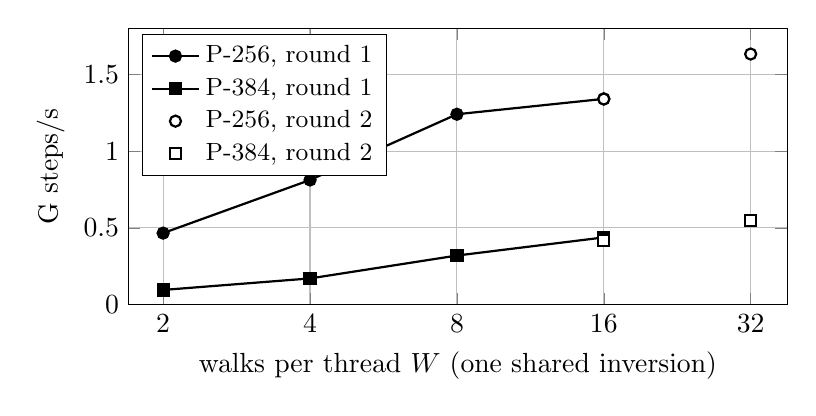
\begin{tikzpicture}
\begin{axis}[
  width=0.82\textwidth,
  height=0.42\textwidth,
  xlabel={walks per thread $W$ (one shared inversion)},
  ylabel={G steps/s},
  xmode=log, log basis x=2,
  xtick={2,4,8,16,32},
  xticklabels={2,4,8,16,32},
  xmin=1.7, xmax=38,
  ymin=0, ymax=1.8,
  grid=major,
  legend style={at={(0.02,0.98)},anchor=north west,font=\small},
]
\addplot[mark=*,thick] coordinates {
  (2,0.466) (4,0.812) (8,1.24) (16,1.340)
};
\addlegendentry{P-256, round 1}
\addplot[mark=square*,thick] coordinates {
  (2,0.096) (4,0.171) (8,0.32) (16,0.438)
};
\addlegendentry{P-384, round 1}
\addplot[mark=*,only marks,mark options={fill=white},thick] coordinates {
  (16,1.339) (32,1.632)
};
\addlegendentry{P-256, round 2}
\addplot[mark=square*,only marks,mark options={fill=white},thick] coordinates {
  (16,0.417) (32,0.548)
};
\addlegendentry{P-384, round 2}
\end{axis}
\end{tikzpicture}
\caption{The NIST rho walk on one RTX~PRO~6000 at 256 threads per block,
  PTX build, unrestricted registers, against the batch width $W$.
  Filled markers are the round-1 sweep, open markers the round-2 sweep
  with the by-reference inversion and the $W=32$ instance. Each point
  is one cell of $8{,}192$ iterations; distinguished-point counts
  matched the $2^{-24}$ rate in every cell.}
\label{fig:nist-w}
\end{figure}

\subsection{What carried over and what did not}
\label{sec:nist-lessons}

Three of the ECC2K-130 levers transferred directly. Native carry
handling, batch width and the refusal of register caps all moved the
NIST walk in the same direction they moved the binary one, and the
combined effect was $1.52\times$ on P-256 and $2.61\times$ on P-384 over
the first working build. The size of each lever did not transfer. The
batch width, a modest knob on ECC2K-130, was the largest single factor
here because a prime-field inversion takes some forty times as many
multiplications as a normal-basis one. Launch geometry, a real gain on the
binary walk, was nearly flat. In other words the ladder carried over,
but its rungs were spaced differently, and the only way to find the
spacing was to measure it.

The comparison also puts the two walks on one scale. On the same card
the ECC2K-130 campaign build runs $14.64$ billion complete iterations
per second and the best P-256 walk $1.63$ billion steps, a factor of
about nine. A 131-bit binary product is six \texttt{CLMAD}
instructions; a 256-bit prime product is two hundred or so
carry-chained integer instructions (Table~\ref{tab:fp256}). That
factor of nine is the carry-less unit's advantage made concrete.

The obvious next rungs are the ones the round-2 record names: a $W=64$
instance (which will spill at the register ceiling and probably lose,
but is worth one cell to confirm), reseeding off the critical path,
and a second walk per step from the same table read. A repeated,
interleaved pairing of the best cell against its control, in the
style of Section~\ref{sec:gpu}, would also turn these single-run
ratios into intervals. None of that changes the exponent, and none of
it is meant to.
